\documentclass[12pt]{article}
\usepackage{placeins}
\usepackage[
singlelinecheck=false % <-- important
]{caption}
\usepackage{graphicx}
\usepackage{multirow}
\usepackage{outlines}
\usepackage{enumitem}
\usepackage{alltt}%
\usepackage{csquotes}
\usepackage{anysize}
\usepackage{amsmath}
\usepackage{mathtools}
\usepackage{bbm}
\usepackage{booktabs}
\usepackage{tabularx}
\usepackage[usenames]{xcolor}
\usepackage[nohead]{geometry}
\usepackage[doublespacing]{setspace}  %set square brackets to singlespacing or doublespacing
\usepackage[bottom]{footmisc}
\usepackage{indentfirst}
\usepackage[labelfont=bf]{caption}
\usepackage{authblk}
\usepackage{natbib}
\usepackage{subfig}
\usepackage[section]{placeins}
\usepackage[flushleft]{threeparttable}
\usepackage{endnotes}
\usepackage{rotating}
\usepackage{datetime}
\usepackage{bibentry}
\usepackage{wrapfig}
\usepackage{siunitx}
\usepackage{times}    %Times New Roman
\usepackage[urlcolor=blue,citecolor=blue,linkcolor=blue,colorlinks=true]{hyperref}
		%see http://en.wikibooks.org/wiki/LaTeX/Hyperlinks

\usepackage{dcolumn}  %decimal aligned columns
\newcolumntype{d}[1]{D{.}{\cdot}{#1} }
%the argument for d specifies the maximum number of decimal places

\newdateformat{mydate}{\monthname[\THEMONTH] \THEYEAR}
\geometry{left=1in,right=1in,top=1.00in,bottom=1.0in}
\marginsize{1 in}{1 in}{1 in}{1 in}
\setlength{\textfloatsep}{0.1cm}
\setlength{\floatsep}{1cm}
\renewcommand\floatpagefraction{.9}
\renewcommand\topfraction{.9}
\renewcommand\bottomfraction{.9}
\renewcommand\textfraction{.1}  
\renewcommand\Affilfont{\fontsize{10}{10.8}\itshape}   %changes font of affiliations
\newcommand{\jcomment}[2]{\hspace{0in}#2}  %custom, found on  web, to ignore everything in between, for commenting.

\title{EconS 581 Assignment 3: Stated Preference}
\author[1]{Tiana Randriamaro}
\date{\today}
\begin{document}
  \maketitle
\singlespace
\textbf{Econometrics}
\begin{enumerate}
\item Using the Kolkata vaccine dataset, estimate WTP using a parametric (probit) model for cholera and typhoid vaccines in the two neighborhoods, with and without TTT.  Estimate a model without covariates, and then a model that includes a dummy for gender (male), dummies for education levels (edu2 edu3 edu4), respondent age (age) and a dummy for whether the respondent knows someone who has had the disease (KNOW).  Calculate mean expected WTP for the following, for the two neighborhoods (Beliaghata and Tiljala) separately: Cholera No Time to Think, Cholera Time to Think.\\

\textbf{WTP for cholera and typhoid vaccines in the two neighborhoods with and without TTT}\\
Using the probit model, I estimate the coefficients for price, neighborhood, and time to think. Then, I replace the time to think variable by 0 for without time to think and 1 with time to think. The WTP is defined as 
\[ WTP_j = \frac{\alpha*Z_j}{\beta_p} + \frac{\epsilon_j}{\beta_p} \]
where $\alpha$ is the vector of coefficients and $Z_j$ is the vector of variables except the price. The expectation is 
\[ E [WTP_j \mid \alpha,\beta,Z_j ] = \frac{\alpha*Z_j}{-\beta_p}=\frac{-.294ttt - .387til + .844}{0.003} \]
\begin{itemize}
\item $WTP$ without time to think $ = 237.49$.
\item $WTP$ with time to think $ = 154.67$ 
\end{itemize}
This means that if people are given some time to think, their willingness to pay decreases and they would not want to pay for the vaccine.\\
The model estimated without covariates is reported as model (1) in Table 1. All of the coefficients are negatives except for the constant term. The higher the referendum price, the less likely the respondent is to say yes for the vaccines. The opportunity for time to think also negatively affect the likelihood of respondents to say yes to vaccines and finally, being in the Tiljala neighborhood reduces the likelihood of respondents to get the vaccines. All of the coefficients are statistically significant. The estimated WTP for this model is $WTP = 237.48$.\\
The model estimated with dummy variables for gender, education levels, and whether the respondent knows someone who has had the disease is model (2) in Table 1. The estimated WTP for this model is $WTP = 326.79$. The coefficients on price, time to think, Tiljala, and male are negatively affecting the likelihood of respondents to get a vaccine. Being  young (less than 25 years old) also increases the likelihood of getting a vaccine as well as all levels of education and knowing someone who has had the disease. Being young, male and residing in Tiljala are not statistically significant in determining the model.\\
In Table 2, I am reporting the expected willingness to pay per neighborhood. I used the same formula as defined above and used the model with covariates. I also used the same method in calculating the $WTP$. I first estimated the probit model, then to get each of the category, I replaced $ttt$ to 0 for no time to think and 1 for time to think, $chol$ is 0 for typhoid and 1 for cholera, $til$ set to 0 for Beliaghata and 1 for Tiljala.\\
\FloatBarrier
\begin{table}[h]  
\caption{Probit model results}
{\label{tab:probit}}
\small
{
\def\sym#1{\ifmmode^{#1}\else\(^{#1}\)\fi}
\begin{tabular}{l*{2}{c}}
\hline\hline
            &\multicolumn{1}{c}{(1)}&\multicolumn{1}{c}{(2)}\\
            &\multicolumn{1}{c}{yesno}&\multicolumn{1}{c}{yesno}\\
\hline
yesno       &                     &                     \\
pricRs      &    -0.00356\sym{***}&    -0.00380\sym{***}\\
            &  (0.000263)         &  (0.000278)         \\
[1em]
ttt         &      -0.294\sym{*}  &      -0.334\sym{**} \\
            &     (0.118)         &     (0.122)         \\
[1em]
til         &      -0.388\sym{**} &      -0.148         \\
            &     (0.118)         &     (0.129)         \\
[1em]
male        &                     &     -0.0480         \\
            &                     &     (0.102)         \\
[1em]
young       &                     &       0.152         \\
            &                     &     (0.169)         \\
[1em]
edu2        &                     &       0.548\sym{***}\\
            &                     &     (0.140)         \\
[1em]
edu3        &                     &       0.940\sym{***}\\
            &                     &     (0.167)         \\
[1em]
edu4        &                     &       0.914\sym{***}\\
            &                     &     (0.199)         \\
[1em]
KNOW        &                     &       0.211\sym{*}  \\
            &                     &     (0.100)         \\
[1em]
\_cons      &       0.844\sym{***}&       0.150         \\
            &    (0.0918)         &     (0.156)         \\
\hline
\(N\)       &         826         &         826         \\
\hline\hline
\multicolumn{3}{l}{\footnotesize Standard errors in parentheses}\\
\multicolumn{3}{l}{\footnotesize \sym{*} \(p<0.05\), \sym{**} \(p<0.01\), \sym{***} \(p<0.001\)}\\
\end{tabular}
}

\end{table}

\begin{table}[h]
\caption {Expected WTP}
%\centering
\begin{tabular}{c c c c c}
\hline\hline
E[WTP] &  Cholera NTT &  Cholera TTT & Typhoid NTT & Typhoid TTT  \\ [0.5ex] % inserts table %heading
\hline
Tiljala & 277.35 &189.45 & 311.43 & 223.53\\
Beliaghata &315.60 &227.71 & 349.68 & 261.79 \\ [1ex]
\hline
\end{tabular}
\label{table:wtp}
\end{table}
\FloatBarrier

\item Using the Vietnam choice dataset, estimate a conditional logit model of vaccine demand ignoring (pooling together) the two TTT treatments.  Then test whether TTT affects parameter estimates.  Do this by first running models separately and then by interacting all coefficients and using Wald tests.  Do you reach the same conclusions about whether TTT affects parameters?  Calculate part-worth WTP estimates for increasing duration and effectiveness.\\

In Table 3, I have the results from the conditional logit model of choice of vaccine for the Vietnam choice dataset. In the first model, I am ignoring the two $ttt$ treatments, I find that $price$, $asc$ (preference for status-quo or no vaccine), vaccine choice, and effectiveness of vaccine at $99\%$ are statistically significant. In the second model, I made an interaction between the explanatory variables and the time to think $ttt$. The coefficients for $price,eff99,vacc_ch,asc$  remain statistically significant and of the sign as each parameter in the first model. The interaction variables $tttprice$ and $tttasc$ are statistically significant meaning that the time to think treatment affects both price and the tendency to prefer status-quo. Wald tests for the parameters for interacted vs. non-interacted variables resulted in coefficients for $asc$ statistically different from $tttasc$ and $eff99$ statistically different from $ttteff99$. With the hypothesis of interacted parameters equal to non-interacted parameters, only $asc$ and $eff99$ resulted in p-value that allow for rejecting the null hypothesis. For the other parameters, I fail to reject the null.\\
\[Null \quad Hypothesis: asc - tttasc = 0\]
\begin{align}
    chi2(1) & = 21.28 \\
    Prob > chi2 & = 0.0000
\end{align}
\[Null \quad Hypothesis: eff99 - ttteff99 = 0\]
\begin{align}
    chi2(1) & = 15.78 \\
    Prob > chi2 & = 0.0001
\end{align}
The part-worth $WTP$ is defined as 
\[ WTP = \frac{\beta_q}{-\beta_p} \]
Here, the $WTP$ for increasing the duration of effectiveness is measured as 
\[ WTP = \frac{\beta_{dure20}}{-\beta_p} = \frac{0.0436}{0.0865} = 0.504 \]
The $WTP$ for increasing effectiveness from current effectiveness at $\%70$ is 
\[ WTP = \frac{\beta_{eff70}}{-\beta_p} = \frac{0.000570}{0.0865} = 0.006 \]
and for current effectiveness at $\%99$
\[ WTP = \frac{\beta_{eff99}}{-\beta_p} = \frac{0.798}{0.0865} = 9.22 \]
\FloatBarrier
\begin{table}[h]  
\caption{Conditional logit model results}
{\label{tab:condlogit}}
\small
{
\def\sym#1{\ifmmode^{#1}\else\(^{#1}\)\fi}
\begin{tabular}{l*{2}{c}}
\hline\hline
            &\multicolumn{1}{c}{(1)}&\multicolumn{1}{c}{(2)}\\
            &\multicolumn{1}{c}{choice}&\multicolumn{1}{c}{choice}\\
\hline
alternative &                     &                     \\
price       &     -0.0865\sym{***}&     -0.0632\sym{***}\\
            &   (0.00663)         &   (0.00868)         \\
[1em]
eff70       &    0.000570         &     -0.0615         \\
            &    (0.0446)         &    (0.0601)         \\
[1em]
eff99       &       0.798\sym{***}&       0.729\sym{***}\\
            &    (0.0454)         &    (0.0613)         \\
[1em]
dure20      &      0.0436         &      0.0362         \\
            &    (0.0311)         &    (0.0417)         \\
[1em]
vacc\_ch     &       0.131\sym{***}&       0.123\sym{**} \\
            &    (0.0289)         &    (0.0383)         \\
[1em]
asc         &      -0.109\sym{*}  &      -0.339\sym{***}\\
            &    (0.0519)         &    (0.0754)         \\
[1em]
tttprice    &                     &     -0.0549\sym{***}\\
            &                     &    (0.0136)         \\
[1em]
ttteff70    &                     &       0.139         \\
            &                     &    (0.0901)         \\
[1em]
ttteff99    &                     &       0.171         \\
            &                     &    (0.0919)         \\
[1em]
tttdure20   &                     &      0.0111         \\
            &                     &    (0.0629)         \\
[1em]
tttvacc\_ch  &                     &      0.0202         \\
            &                     &    (0.0585)         \\
[1em]
tttasc      &                     &       0.434\sym{***}\\
            &                     &     (0.105)         \\
\hline
\(N\)       &        7200         &        7200         \\
\hline\hline
\multicolumn{3}{l}{\footnotesize Standard errors in parentheses}\\
\multicolumn{3}{l}{\footnotesize \sym{*} \(p<0.05\), \sym{**} \(p<0.01\), \sym{***} \(p<0.001\)}\\
\end{tabular}
}

\end{table}
\FloatBarrier

\item Estimate a mixed logit model allowing the coefficient on $price$ and the $asc$ to be normally distributed but other parameters as fixed coefficients. Plot the distribution of predicted coefficients (preferences) for the two random parameters (mixlbeta).\\

Table 4 contains the estimated mixed logit model with the coefficient on $price$ and $asc$ normally distributed. The coefficient means are reported and the standard deviations. The mean coefficient on $dure20$, $vacc_ch$,$price$, and $asc$ are statistically significant with the mixed logit.\\
Below are the distribution plots of the individual-level parameters for $price$ and $asc$.The distribution of individual $price$ coefficient is close to a normal distribution but it is skewed to the right. The distribution of individual $asc$ coefficient does not appear to form a normal distribution.\\

\begin{table}[h]  
\caption{Mixed logit model results}
{\label{tab:mixlogit}}
\small
{
\def\sym#1{\ifmmode^{#1}\else\(^{#1}\)\fi}
\begin{tabular}{l*{1}{c}}
\hline\hline
            &\multicolumn{1}{c}{(1)}\\
            &\multicolumn{1}{c}{choice}\\
\hline
Mean        &                     \\
eff70       &     0.00898         \\
            &    (0.0607)         \\
[1em]
eff99       &       1.452\sym{***}\\
            &    (0.0782)         \\
[1em]
dure20      &       0.166\sym{**} \\
            &    (0.0511)         \\
[1em]
vacc\_ch     &       0.186\sym{***}\\
            &    (0.0400)         \\
[1em]
price       &      -0.270\sym{***}\\
            &    (0.0280)         \\
[1em]
asc         &      -1.162\sym{***}\\
            &     (0.253)         \\
\hline
SD          &                     \\
price       &       0.316\sym{***}\\
            &    (0.0300)         \\
[1em]
asc         &       4.259\sym{***}\\
            &     (0.334)         \\
\hline
\(N\)       &        7200         \\
\hline\hline
\multicolumn{2}{l}{\footnotesize Standard errors in parentheses}\\
\multicolumn{2}{l}{\footnotesize \sym{*} \(p<0.05\), \sym{**} \(p<0.01\), \sym{***} \(p<0.001\)}\\
\end{tabular}
}

\end{table}

\begin{figure}[htbp]
\centering
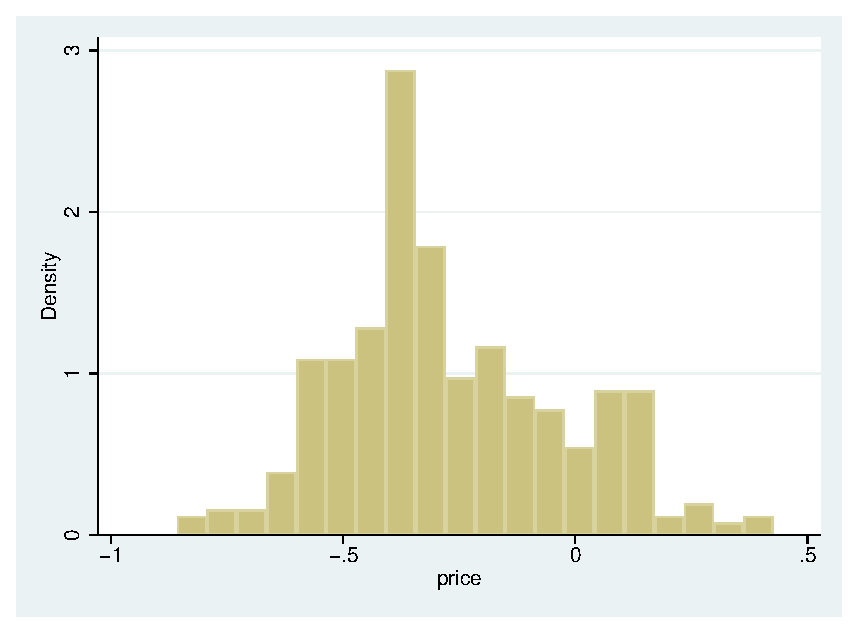
\includegraphics[width=4.9in]{pricegraph.eps}
\caption{Distribution of predicted price coefficient}
\label{price}
\end{figure}

\begin{figure}[htbp]
\centering
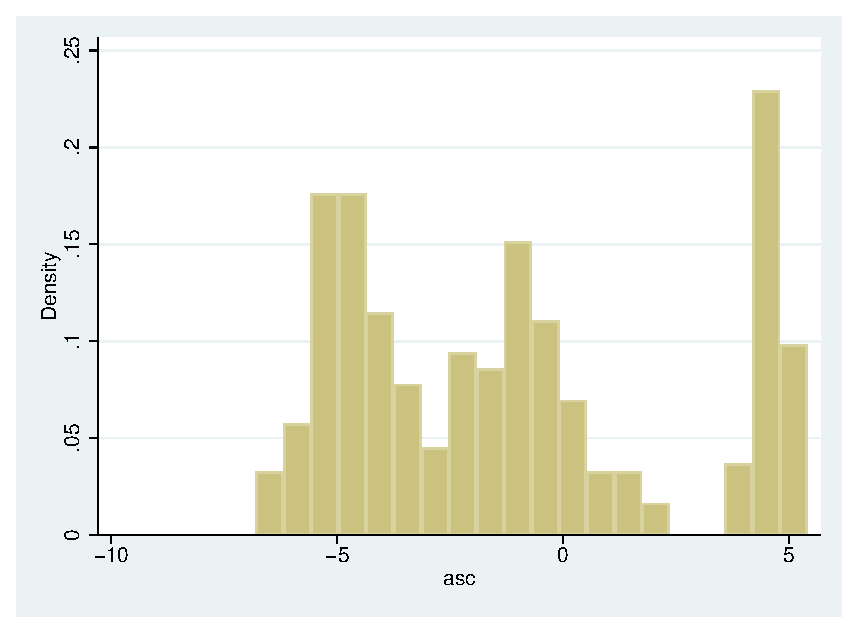
\includegraphics[width=4.9in]{ascgraph.eps}
\caption{Distribution of predicted asc coefficient}
\label{price}
\end{figure}


\end{enumerate}

\end{document}
